\documentclass{article}

\usepackage{graphicx}
\usepackage[utf8]{inputenc}
\usepackage[T1]{fontenc}
\usepackage[francais]{babel}
\usepackage{hyperref}
\usepackage{amsmath,amsfonts,amssymb}
\usepackage{Tkz-Tab}
\usepackage{wrapfig}
\usepackage{verbatim}
\usepackage{array}

\begin{document}

\title{Gestion de flux dans le réseau
	\smallbreak
	TD n\degre4
	\smallbreak
	Modélisation mathématique
	\smallbreak
	Q4}
\author{Sibylle Roux \and Juliette Arazo \and Nicolas Le Gallo \and Tanguy Thomas}


\maketitle

\newpage

\tableofcontents

\newpage

\part{Etude statistiques des temps interarrivés}

\section{Etude statistique des temps interarrivés pour tous les serveurs}

\subsection{Indicateurs de position et de dispersion}

\begin{tabular}{|c|c|c|c|}
  \hline
  Indicateurs & Serveur 1 & Serveur 2 & Serveur 3 \\
  \hline
  Minimum & 0.01 & 0.04 & 0.01 \\
  Maximum & 134 & 88.9 & 68.6 \\
  Etendue & 134 & 88.9 & 68.6 \\
  Moyenne & 15.5 & 10.6 & 6.27 \\
  Médiane & 11.5 & 6.82 & 4.35 \\
  Q1 & 5.05 & 3.29 & 1.75 \\
  Q3 & 21.9 & 13.9 & 8.36 \\
  IQ & 16.8 & 10.6 & 6.61 \\
  Ecart-Type & 15 & 11.3 & 6.85 \\
  Variance & 225 & 127 & 46.9 \\
  \hline
\end{tabular}

\subsection{Fonction de répartition}

\subsection{Histogramme}

\part{Etude statistiques des temps de service}

\section{Indicateurs de positions et de dispersions}

\section{Fonctions de répartition}

\section{Histogrammes}

\paragraph{Histogramme}
\begin{center}
%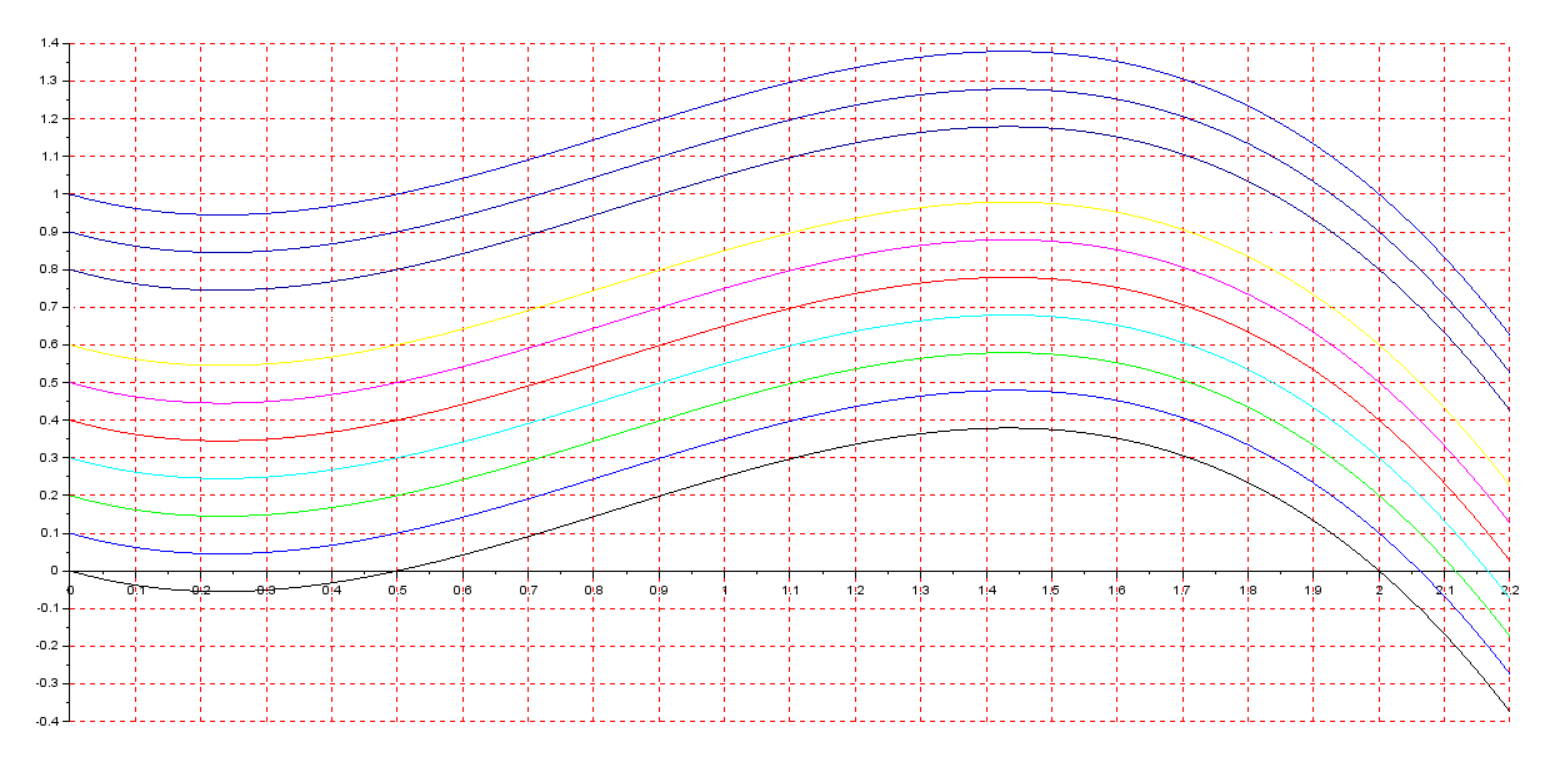
\includegraphics[width=300px]{img/part1/AlleeI.png}
\end{center}
\paragraph{}

\part{Ajustement graphique à des lois mathématique}

\section{Tous les serveurs}

\subsection{Ajustement à la loi uniforme}

\subsubsection{Estimation des paramètres}
\subsubsection{Superposition de la fonction de répartition}
\subsubsection{Superposition de la fonction de densité et de l'histogramme}

\subsection{Ajustement à la loi normale}

\subsubsection{Estimation des paramètres}
\subsubsection{Superposition de la fonction de répartition}
\subsubsection{Superposition de la fonction de densité et de l'histogramme}

\subsection {Ajustement à la loi exponentielle}

\subsubsection{Estimation des paramètres}
\subsubsection{Superposition de la fonction de répartition}
\subsubsection{Superposition de la fonction de densité et de l'histogramme}

\section{Serveur 1}

\subsection{Ajustement à la loi uniforme}

\subsubsection{Estimation des paramètres}
\subsubsection{Superposition de la fonction de répartition}
\subsubsection{Superposition de la fonction de densité et de l'histogramme}

\subsection{Ajustement à la loi normale}

\subsubsection{Estimation des paramètres}
\subsubsection{Superposition de la fonction de répartition}
\subsubsection{Superposition de la fonction de densité et de l'histogramme}

\subsection {Ajustement à la loi exponentielle}

\subsubsection{Estimation des paramètres}
\subsubsection{Superposition de la fonction de répartition}
\subsubsection{Superposition de la fonction de densité et de l'histogramme}

\section{Serveur 2}

\subsection{Ajustement à la loi uniforme}

\subsubsection{Estimation des paramètres}
\subsubsection{Superposition de la fonction de répartition}
\subsubsection{Superposition de la fonction de densité et de l'histogramme}

\subsection{Ajustement à la loi normale}

\subsubsection{Estimation des paramètres}
\subsubsection{Superposition de la fonction de répartition}
\subsubsection{Superposition de la fonction de densité et de l'histogramme}

\subsection {Ajustement à la loi exponentielle}

\subsubsection{Estimation des paramètres}
\subsubsection{Superposition de la fonction de répartition}
\subsubsection{Superposition de la fonction de densité et de l'histogramme}

\section{Serveur 3}

\subsection{Ajustement à la loi uniforme}

\subsubsection{Estimation des paramètres}
\subsubsection{Superposition de la fonction de répartition}
\subsubsection{Superposition de la fonction de densité et de l'histogramme}

\subsection{Ajustement à la loi normale}

\subsubsection{Estimation des paramètres}
\subsubsection{Superposition de la fonction de répartition}
\subsubsection{Superposition de la fonction de densité et de l'histogramme}

\subsection {Ajustement à la loi exponentielle}

\subsubsection{Estimation des paramètres}
\subsubsection{Superposition de la fonction de répartition}
\subsubsection{Superposition de la fonction de densité et de l'histogramme}

\newpage
\appendix

\section{}

\subsection{}

\subsubsection{}

\begin{verbatim}
\end{verbatim}

\end{document}